\documentclass{cmspaper}
\begin{document}

%==============================================================================
% title page for few authors

\begin{titlepage}

% select one of the following and type in the proper number:
   \cmsnote{2005/TBD}
%  \internalnote{2005/000}
%  \conferencereport{2005/000}
   \date{\today}

  \title{DRAFT Technical Design of the Dataset Bookkeeping Service DRAFT}

  \note{Draft Version v0\_5}

  \begin{Authlist}
    M. Anzar Afaq, Lothar Bauerdick, Greg Graham, Vijay Sekhri, Igor Terekhov, 
    Yujun Wu
       \Instfoot{fnal}{Fermi National Accelerator Laboratory}
    Lassi Tuura
       \Instfoot{ne}{Northeastern Unversity, Boston, MA, USA}
    Peter Elmer
       \Instfoot{prince}{Princeton University, Trenton, NJ, USA}
    Tim Barrass
       \Instfoot{bristol}{University of Bristol, Bristol, UK}
  \end{Authlist}

\collaboration{for the CMS collaboration}

  \begin{abstract}
      This note describes the Dtaaset Bookkeeping Service (DBS) prototype for the 
  CMS Data Management (DM) project.  The scope of the DBS is to provide a tools to 
  store information about real and simulated CMS data in a queriable format.  The
  supported queries should allow physicists and their agents to discover what 
  data is available, subject to given constraints, to retrieve information 
  about specific data and to define derived (``analysis'') datasets. This note
  contains some use cases and requirements to be fulfilled by such a system.  
  An Entity-Relationship diagram (conceptual schema) is presented for implementation 
  of the system.
  \end{abstract} 

  
\end{titlepage}

\setcounter{page}{2}%JPP

\section{Introduction}

The Dataset Bookkeeping Service (DBS) is designed to be the part of the
CMS Data Management which hosts the attributes describing the actual event data
(and some associated entities). It will contain sufficient information
to discover, define and use for processing pieces of CMS data,
such as {\em datasets} and other entities described herein.

The purpose of this document is to define DBS in sufficient detail as to
be able to build this component as part of the Baseline Data Management
System described elsewhere \cite{dmman}. To do so, we start with making
 certain detailed ``operating assumptions'' about the CMS data organisation, 
based on the higher-level documents of 
Data Management RTAG\cite{rtag7} and the CMS Computing Model\cite{CM}.
We then include (by reference?) a set of use cases derived from
our experiences. Finally, we assume that we will use a relational 
database management system (RDBMS) for a persistent storage
of all this information and design a {\it schema} 
that represents entities introduced
here and relations thereof. 

Access to CMS data should take place through interfaces designed for an 
appropriate level of abstraction for the physicist.  The physicist is not 
interested in implementation details, such as files or transport mechanisms. 
In fact, we expect that much of the schema will be hidden from the physicist
as well by the properly designed (and implemented!) interfaces.

The dataset bookkeeping service (DBS) should not include functionality that could in 
principle be delivered by other services.  The schema design should therefore make 
reference to external databases or services as required.  It should 
concentrate on supporting the decomposition of datasets into event collections, finding the 
components needed to analyze or to transfer an event collection, and the attributes 
needed to support a sensible level of dataset discovery service.  


%It was taken as an operating assumption that POOL can be considered to be a service that 
%exists for the duration of a running application only.  The DBS may contain POOL contact 
%information, but will not rely on POOL itself to run queries or for replica information.

\section{Refining the Data Organisation}

\begin{figure}[hbtp]
  \begin{center}
    \resizebox{10cm}{!}{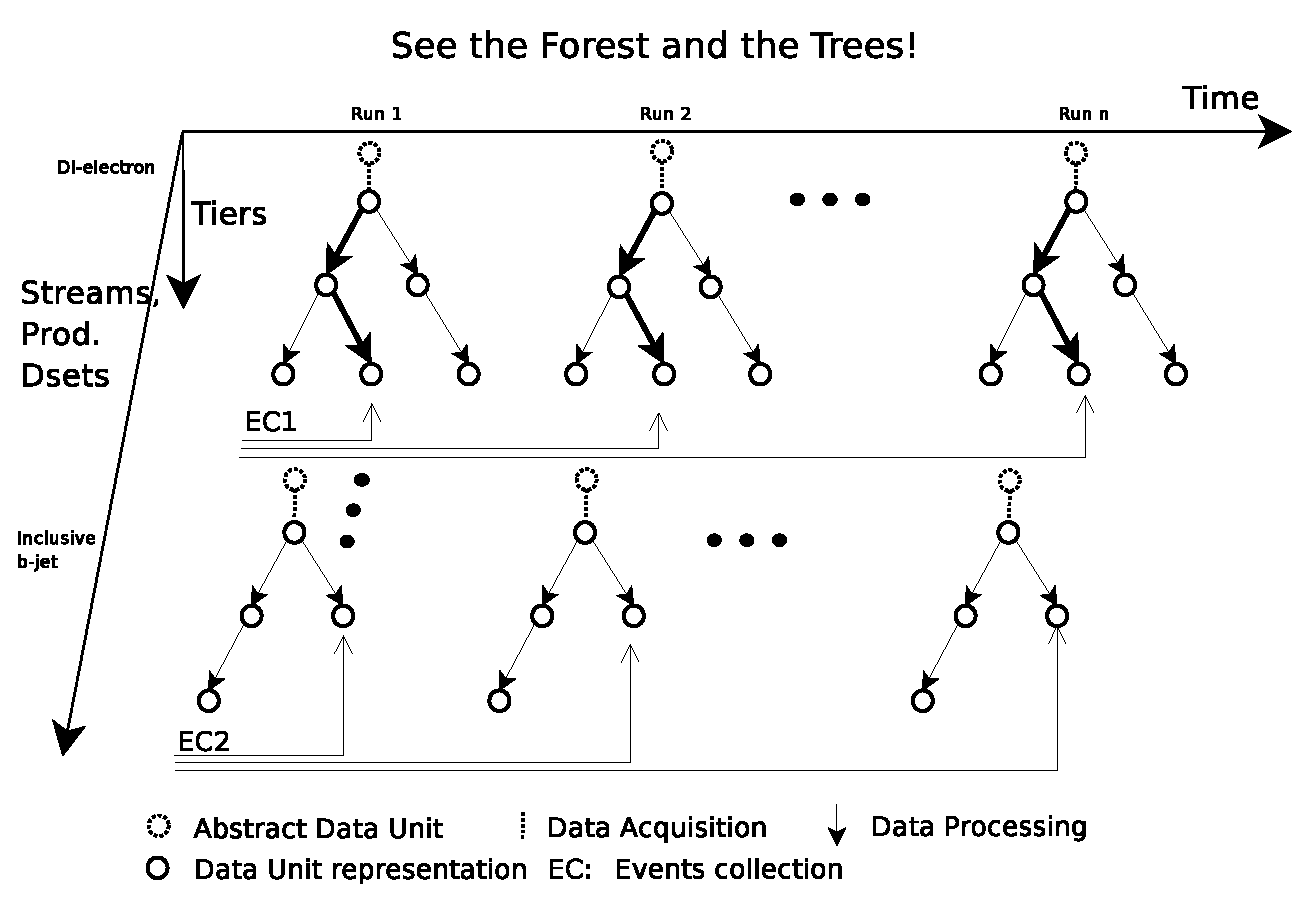
\includegraphics{forest.eps}}
    \caption{The figure shows a forest of trees.  The root of each tree is a 
chunk of data defined by some criterion, such as run number and trigger condition.
The path to each node in the tree represents the result of processing that 
data through a particular sequence of processing steps.  Each node is called 
a ``data unit representation''.  There can be trees in different Primary Datasets (along the 
axis pointing out of the page) and there can be Event Collections comprising nodes 
within each Primary Dataset that have the same processing path. An Event Collection 
that contains all possible like-path nodes in a Primary Dataset is a Dataset 
Representation.}
    \label{fig:forest}
  \end{center}
\end{figure}

The following terms have been identified as being at an appropriate level 
of abstraction:

\begin{itemize}
\item {\bf Primary Dataset}. The basic category of analyzability, distinguished informally 
by grouping data into groups that share the same generation parameters in the case on Monte
Carlo or the same trigger/stream definitions in the case of real data.
\item {\bf Dataset}. The basic category of homogeneity, distinguished informally 
by grouping data into groups that could ordinarily be read as input by the same application 
in the same job.  Items belonging to the same dataset will share attributes such as 
processing parameters used in the creation of the dataset. This entity is also known as 
``Dataset Representation'' because of the close association to the entity 
Representation (see below). 
\item{\bf Data Unit Representation}
 This represents the results of processing of a well defined data unit 
(chunk of events) belonging to the same dataset through a well defined sequence of processing steps.
The data inside of a representation could for example correspond to a ``run'' but it 
does not have to.  It could correspond to a luminosity segment within a run.  This is 
the entity which we will relate to logical files.
\item {\bf Event Collection} This represents an arbitrary collection of representations within 
the same dataset that have gone through equivalent processing steps.  The goal of the 
analysis user or his/her agent is to use the DBS to discover and select an event 
collection for analysis.\footnote{The Event Collection entity can contain both the concepts of 
an Analysis Dataset as described in the RTAG, as well as the results of a skim.}
\end{itemize}

We attempt to present these entities in Figure \ref{fig:forest}.  A more precise definition
of these entities in terms of subsets of the data appears in the Addendum.

In contrast to the above abstractions, objects like files and sites are 
of interest to the system underlying the dataset bookkeeping service and are considered 
implementation details.  While we must keep track of such objects as well, 
files and filenames should not contain physics metadata.  It will therefore
be of interest later on how the abstractions above are related to actual OS 
supported objects like files.  It was furthermore decided not to make special 
accounting for special files, like the ``META'' files, that currently exist in the 
CMS event data model (EDM) but are not intrinsic.  It is assumed that the EDM group will 
make changes in the way data is written in CMS so that the number of special files tends 
to zero in the long run.  

The skeletal Entity-Relationship (ER) view onto this model is
shown in Figure \ref{fig:highlevel}. We will discuss it further when
we proceed to a the schema design after listing some important use
cases.  Note that metadata/attribute support tables are not shown 
in figure 2. Attributes that are mapped to the entities shown can be 
stored on table or in supporting tables.

\begin{figure}[hbtp]
  \begin{center}
    \resizebox{6cm}{!}{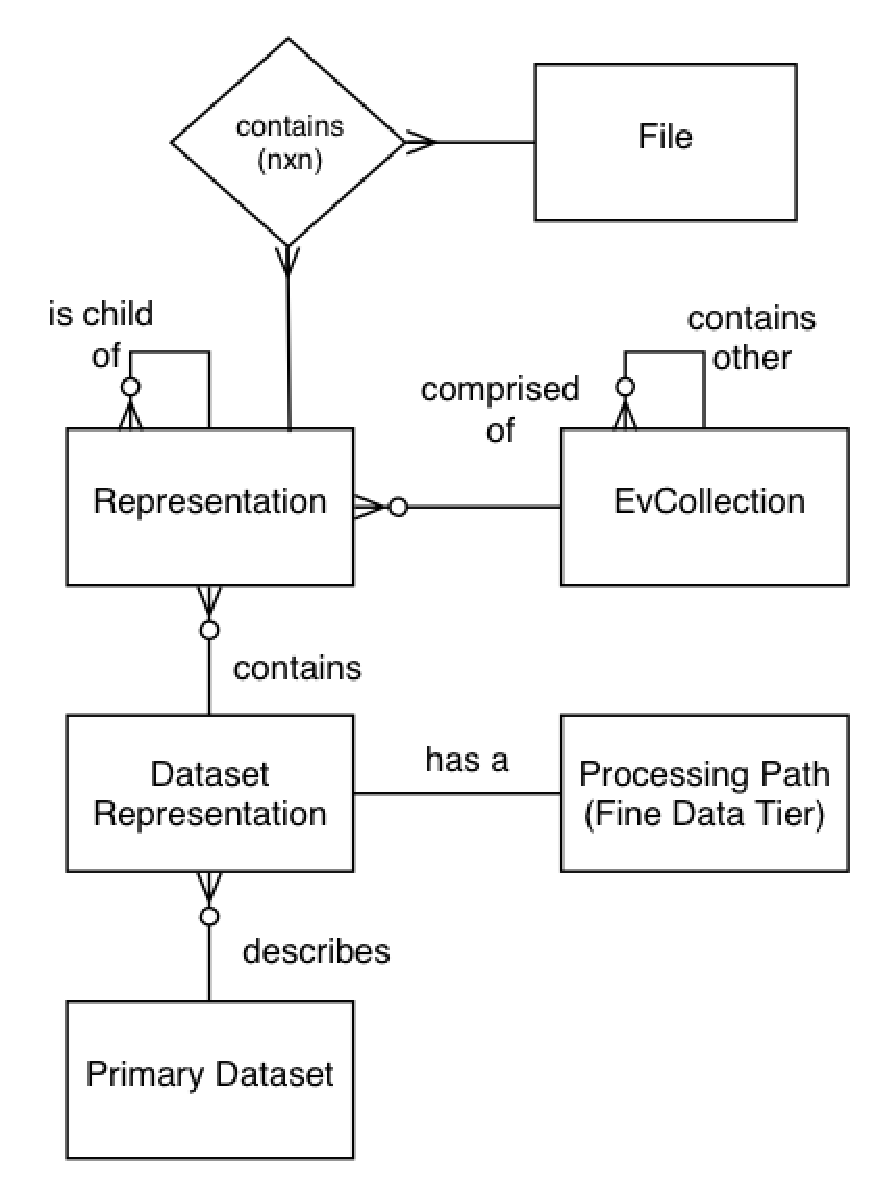
\includegraphics{DatasetBookkeeping-1a.eps}}
    \caption{Basic outline of the core DBS schema including the basic entities outlined 
in the Introduction: Primary Dataset, Dataset Representation, Representation, 
and Event Collection.  A few other supporting entities are shown as well.  Representation 
is mapped $N$ to $N$ with Logical Files. }
    \label{fig:highlevel}
  \end{center}
\end{figure}


\section{Scenarios, Use Cases, and Example Queries}

In this Section, we explore the most frequent use cases: data import
({\em putting} data into the system), queries ({\em seeing} what is there),
and workflow for read access ({\em getting} data out of the system).

\subsection{Data import}

Even though data will probably be produced one file at a time, its import  
into the data management system is probably best done in terms of the 
more abstract Representation entity. We imagine the 
following scenario to put  a Representation 
into the system in such a way that supports streaming.

\begin{itemize}
\item An agent is in possession of files associated with a Representation
containing real data.
\item The agent utilizes an API method addToDataset(*dataInfo).  The dataInfo structure 
will contain information like 
\begin{itemize}
\item Logical Filenames associated with the import
\item Attributes associated with the production of the files, such as 
the latest processing history and input description if not null. 
\end{itemize}
\item The method searches for the best Event Collection to add the Representation to.  
Special Event Collections called ``blocks'' are envisioned for this purpose.  
\footnote{The blocks will have attributes of interest to a data transfer and storage 
system, like maximum size and location information. These are of system interest only.}
It should reconcile the processing history with existing processing paths and 
open a new Dataset Representation if necessary.
\begin{itemize}
\item If there is an open block, the run is added to the open block.
\item If there is no open block, a new open block is created and the run added to that one.
\item If the new block size is greater than the max block size, the block is closed.  
\end{itemize}
\end{itemize}

In order for this to work without a potentially complex synchronization system, 
open blocks should not be transportable. Streaming is of obvious concern here, 
and there is a tension between wanting to keep the blocksize small enough so that 
new data can be transferred to interested sites quickly and large enough to satisfy 
the needs of data management.

Alternatively, data can be streamed file by file; but in that case we need to synchronize
open blocks between sites sharing the particular data.

\subsection{User Queries}

Below we explore user queries corresponding to the various access modes,
and subsequently attempt to generalize. Among the goals of this discussion
is clarification of the role of a ``run''.

\subsubsection{Use case 1: Detector Expert}

  The first use case for selecting on run(s) is detector studies, calibrations
and data quality. Note that we are not talking about how the time-varying 
calibrations/conditions are stored and accessed by applications from the 
conditions database itself, but merely how someone doing such studies would 
find the event data to do such studies (i.e. the task of the dataset 
bookkeeping). The common paradigm in HEP is that this is done in terms
of runs, so most likely the person could be (very generically) doing things 
like:
\begin{itemize}
\item coming in the morning, reading the logbook and seeing that there was
     some problem with their subsystem overnight in run NNN (e.g. a crate 
     tripped off or was in some strange state, oddities seen in some 
     monitoring histogram, etc.) and then wanting to look at some raw or 
     rec data with some specialized application to learn more about the
     run quality or problems (often to classify it in a data-quality sense).
\item the detector expert (at some later date) may be trying to determine
     some calibration or corrections. Also in this case it will be natural
     for the expert to ask for different types of data, most typically with
     run ranges. Often what they do may include one component of actually 
     trying to break up the data into run ranges based on the problems and
     state of the detector and one component of actually determining the
     calibrations. 
\end{itemize}

"Run" here represents a natural quantum for thinking about the problem and
the DBS will be asked for data in these terms. Two implications:
\begin{itemize}
\item The DBS will be asked for data (raw, rec and perhaps aod) from particular
    primary datasets with "run" as a selection. This has to be supported and
    some means of configuring jobs at this granularity for at least these
    categories of data must be provided.

\item The "data quality" attributes (good, bad, good for X only, ...) are likely 
    to be specified with a granularity of a single run. These flags may be
    specified for all representations of a particular run's data or just
    for particular ones. (As part of the discussions of the details of how
    "run" is defined, DM should bring this point up explicitly. As it is a 
    relatively common model in HEP, we can probably assume it for the moment.
    See below for further details.)
\end{itemize}

In terms of the schema presented above, run numbers will have to have been 
stored with the Representations.  Possibly, we may have one Representation
per run number within a Primary Dataset.  The use case is satisfied by 
providing query attributes that can identify a Primary Dataset and by 
providing a processing path (null for raw data).  Then, all 
Representations matching the run number can be retrieved and files 
identified corresponding to those Representations.\footnote{In fact, runs 
do not have to be used at all.  The only impportant thing is that the 
basic units of data be distinct and enumerable.  Run number is just a convenient 
illustrative device.}

Note, however, that the fact that data is being asked for using "run" as
the minimal quantum does not imply that the calibrations determined by
the expert need to fall on run boundaries. As we have said that "conditions"
are only read by applications and not the problem of DMS, this should pose no
problems. (Similarly data quality decisions with a finer granularity than 
run, if needed, can be pushed into the conditions database and require 
the use of an application to access them.)  Run status flags can also be used 
if they are imported along with the run numbers when importing Representations.

\subsubsection{Use case 2: Production}
\label{sec:UCprod}

  At the macro level, the production system typically takes something 
as input, e.g. "the raw data from online stream X" and processes it to
produce something like "the aod/rec data for primary dataset X, processed
with orca xyz, etc.". For this use case I'm really considering things
like (re-)reconstruction and aod production.

%  So how are "runs" sometimes used here? 

\begin{itemize}
\item One way to specify the input dataset would be via a run range or list
     of runs (most likely made by selecting on data quality attributes set by
     someone like the expert of use case 1)
\item If the output is intended to be selectable with a "run" granularity,
     in practice the production system may process a given dataset by 
     breaking it up into individual pieces with a granularity such that
     the "run" genealogy of each output can be followed back to an input.
\end{itemize}

  A few things to note:
\begin{itemize}

\item The user may be interested in tracking two types of "history" here:
\begin{itemize}

      \item macro level: how one dataset was transformed to another
      \item micro level: how one "run" representation is mapped to anther one
\end{itemize}

\item The production system is explicitly collaborating in propagating the
    "run" granularity from input to output (and thus allowing it to be
    tracked by the DBS)

\item The use of run ranges and/or run lists explicitly to define the input is 
    partly incidental. If the macro goal of the production system is seen as
    processing one dataset into another, the run-ranges and/or run lists 
    should be captured explicitly in the DBS. I would claim that the proper 
    concept for capturing this is a "dataset" (e.g. as some sort of "dataset 
    tag"). 

\end{itemize}

This use case is supported in much the same way as the last one.  An input 
Primary Dataset and input processing path is given, and then all Representations
matching the run range can be retrieved.  As an additional possibility, an 
Event Collection may be defined as a collection of such Representations and then will 
represent a collection of the corresponding runs.  In terms of tracking the processing
taking place within the Primary Dataset, one interesting effect occurs when 
processing such an event collection.  Even if the framework does not track processing
of individual Representations within an Event Collection, the Representations 
should be loaded into the DBS anyway.  This preserves the structure of tracking 
the processing paths through Representations, and the set of 
files corresponding to the whole processed Event Collection can be assigned to 
each Representation in the derived Event Collection.  The additional cost is that 
the Representation table must be accessed to determine the processing path between 
two Event Collections.  With indexing and the constraint that Event Collections be 
defined only over Representations at the same processing path, this is only a 
constant time inefficiency.


\subsubsection{Use case 3: Analysis End-user}

  The analysis end-user is where things start to get a bit murkier for runs.
From everything written above, runs can and should probably be retained as 
an attribute on which one can easily select.

  That said, somewhere out along the data reduction chain some step (e.g. 
skimming, analysis user "ntuple production", etc.) where the user will
decide (for very practical reasons) to process data representations for more
than one run through some application such that the output no longer has
a 1-1 mapping to "run". See section \ref{sec:createEvColl} for an explanation of how such 
skims can be represented in the schema.


\begin{itemize}
\item the detector expert is still working and may decide (after the 
     analysis-user has already run their analysis over a dataset) that a
     particular run was "bad" after all and should be excluded from their
     end result. (Again assuming that the good/bad granularity is "run", etc.)
\item the detector expert (or some analysis group) may provide some set of
     corrections/updates which the analysis-user needs to apply themselves
     (e.g. they arrived too late to be included in the last re-reconstruction
     or aod production step, or were actually generated from the output of
     the last re-reco or aod production step...). 
\end{itemize}

The DBS and DM should be involved in tracking analysis datasets in which
some mangling has gone on WRT runs, and the relationship of the resulting 
"event collections" to runs becomes significantly more complex, but the 
question here is how much support can/should be provided for selecting on 
things in the DBS by run at that point. (What DBS/DM doesn't do must either 
be done by opening the data in some application which does it or by using 
some application which uses the conditions database, for example, to do the
selection.)

This use case is supported by the Event Collections because the Event Collections 
can be defined over multiple runs and processed through to other event collections
as described in the previous section.  Even if individual runs or Representations 
are not tracked by the user, it is important for the DBS to do so.  In the case 
where multiple jobs are doing the processing, the DBS can be used to keep track of
which pieces have been processed successfully and which have not.  In the case
where there is only one job processing the Event Collection, then it is still 
useful to be able to query and find out which components 
(runs or Representations, it doesn't matter) were processed to 
arrive at the desired result.

%  In the discussion above I've ignored luminosity for the moment. I think the 
%DBS should provide some support for tracking lumi, but I need to catch up on 
%how this is dealt with at hadron machines. More on that later.  

%However, even if the data is sorted into luminosity bins, the luminosity bin
%can serve as the basis for the Representation.

%  I've also completely ignored runs for MC as they are significantly more
%artificial than those for real data since there are far fewer reasons to 
%select MC specifically by "run". What currently defines a "run" for MC in
%CMS? It is defined as the output of a particular batch job.

\subsubsection{Support for Generalized Queries}

%The following queries can be covered in the proposed schema.  In most cases, the 
%queries are straightforward in light of the proposed schema.  As with the diagrams, 
%joins with support tables are omitted in the following for clarity.

Each of the following queries are listed with a short plan for resolving the query.

\begin{itemize}
\item Find all files associated with a Primary Dataset.  Compound join on Primary
Dataset, Dataset Representation, Representation, and File.
  \begin{itemize}
  \item Find all files associated with a run.  Simple join on Representation, File and selection for run number.
  \item Find all files associated with a block.  Compound join on Event Collection, Representation, 
and File.
  \end{itemize}
\item Find all Event Collections associated with a Dataset Representation.  Filtered selection on 
simple join on Event Collection, Representation. (This query caused us to consider that runs 
must belong to distinct datasets, or equivalently that the unique attributes of 
run must include at least both run number and dataset id.  If it is not so, then 
these types of queries become much more complex.)
  \begin{itemize}
  \item Find all assignments associated with a Monte-Carlo Primary Dataset. Filtered selection on join.
  \item Find all blocks and block locations associated with a Dataset Representation. Filtered selection 
  on simple join.
  \end{itemize}
\item Find all data. Unfiltered selection on Primary Dataset.
  \begin{itemize}
  \item Find all data matching a physics criterion.  Filtered selection on dataset or 
  on simple join on dataset, run.
  \item How many are runs in a Dataset Representation.  
Cardinality of simple join on dataset, Representation and selection on run number.
  \item How many events in a dataset.  Selection on dataset.  (This query caused us to 
  consider keeping track of bulk properties such as total number of events that could be 
  updated every time a run is imported.  This could work for luminosity and cross section too.)
  \item Find digitized data corresponding to specific generated data. 
  Filtered selection on Dataset Representation or compound filtered selection of the join of 
Event Collection and Representation.  
  \end{itemize}
\end{itemize}

\subsection{Defining derived datasets}

A user shall be able to define new event collections as ``analysis
datasets''. Some of these datasets will represent the results of processing
of an entire production dataset and will be done on behalf of the entire
collaboration. Others will be defined by groups. Finally, ``private''
datasets defined by individual users for their own consumption may be
supported. We say that such user-defined (aka analysis, aka derived)
datasets have a {\em scope} associated with them.

Some of these derived datasets will also be ``filters'' of their parent
datasets, where the one-to-one relation between a parent and a child
event (representation) is not preserved. It shall therefore be possible
to mark such filtered datasets (sometimes called {\em skims}) appropriately
when defining them.
 
\subsection{Workflow scenario}

We imagine the following workflow building scenario in order to explore the 
interface between data management and workflow management.

\begin{itemize}
\item A physicist wants to create jobs based on data identified by queries against 
the DBS going through the application layer.  A handle to an Event Collection or number N of
Representations is returned.  The details of what is returned should be worked out.
\item Physicist creates $M <= N$ jobs (i.e.- maybe some jobs process 
more than one Representation.)  Job 
creation tool creates jobs in a site independent fashion, knowing only about site 
independent dataset parameters and run numbers etc and instructions for connecting to 
the data (eg- a POOL catalog connection string.)
\item Physicist submits jobs.  Job submission tool consults the DRS through the 
application layer.  Information about sites where the data resides is obtained 
now.  An algorithm (round robin for example) assigns jobs to sites based on where 
corresponding blocks are located.
\item Job files are transferred to the execution site along with the job using e.g. Phedex.
\item The jobs are 'localized' upon transfer to the site.
\item Output data is created and transferred by SRM to the final resting place.
\item The output data is published into the DBS.
\end{itemize}

\section{The Schema}

In order to hide implementation details from the physicist and 
reduce physicist-side overhead, the DBS necessarily needs to keep track of some 
of these details in the backend, so ``file'' is included as a major entity. 
However, the schema proposed here has a progressive view of abstraction 
with file objects at one end, the primary datasets at the other end, and 
intermediate abstractions between them.  The user is presented with the most
abstract concepts first, and consciously has to drill 
down to get to the progressively less and less abstract objects like files.

The ``dressed'' schema is given in Figure \ref{fig:detailed}. We 
would like to first go over the core entities introduced earlier and
shown in Figure \ref{fig:highlevel}.

\subsection{Basic Entities}

Starting at the bottom is the ``Primary Dataset''.  This entity represents a 
set of data that is related in the most general physics way.  
They share attributes that define the kind of data contained in the 
primary dataset, such as generation parameters for Monte Carlo or 
trigger bit information for real data.  The Primary Dataset contains all such
data across all possible processing steps.  

The next layer of abstraction
is the Dataset Representation.  The Dataset Representation is obtained by 
selecting out of the Primary Dataset a particular subset of the data that has been 
processed by a given sequence of application steps.  The sequence is stored 
in a supporting table that stores individual ``processing paths''.  For example,
if a chunk of raw data were processed first by a filter program P1 followed 
by a reconstruction program P2, then the processing path is /P1/P2.  Moreover, 
each component of the path may contain a reference to a distinct record of the 
invocation parameters of the corresponding application and version that did 
the processing\footnote{This is a fine grained example of what is sometimes called
``Data Tier''.  The Data Tier typically contains only information about kind
of application was run.  This has been generalized to contain much more information 
about the processing path.}. 

The next layer of abstraction is the Representation.  The Representation is a 
well defined result set of data obtained by processing a well defined chunk
of data\footnote{A well defined ``chunk'' of data is a set of data that is 
characterized only by the list of event IDs contained therein.} through a 
number of well defined steps.  (see figure \ref{fig:forest}).

The figure shows that a Representation can refer to other representations.  There
are two possibilities which this supports.
\begin{itemize}
\item The Representation contains a reference to its parent. 
\item The Representation may contain references to more than one 
representation in the same processing tree.  
\end{itemize}
The former case can be implemented directly without loops by including the 
full processing path in the unique key of the Representation as well as the 
ID of the root node, or Primary Representation.  The second case may be
supported by a simple mapping table, but the use case is not clear.  For example, 
if the user wants to create an Event Collection consisting of both Hits and 
Digis data in CMS, then the latter construct would be useful.

The Event Collection is a set of Representations that share a processing path.  
Therefore the Event Collection is a way of aggregating a Dataset Representation 
horizontally (i.e.- by event ID) and the Dataset Representation is a way of 
aggregating a Primary Dataset vertically (i.e.- by data content or schema). 
Although the CMS framework may make no distinction there, it is wise in a 
relational database to make such a distinction.  The former is just normal aggregation
of objects into sets, and the latter is specifically needed to model the implicit
OO relationships (e.g.- inheritance) that are possible in the OO framework
but not in an RDBMS. This entity also refers to itself, and this is simply to support
the use case of one user adding to the Event Collection of another user.  Again, this
may be implemented by a simple mapping table.

The following constraints should be applied to the DBS.  These may be included 
later into the schema itself or implemented at a higher software level.
\begin{itemize}
\item[R1]  A Primary Dataset can span data processed by many 
different applications and versions of applications.  
\item[R2] The data contained in a given Representation must 
belong to exactly one Dataset Representation.\footnote{In the appendix, 
and in the schema diagrams, but not yet in the verbage, a Compound 
Representation is also possible which combines more than one path.
However, the Representation entity itself should still follow 
this rule if the Compound Representation is properly contained in the 
self-relationship defined on Representation.}  
\item[R3] An Event Collection should not mix Representations from different 
Primary Datasets.
\end{itemize}

The structure of the schema shows that a Dataset Representation has the same 
structural relationship to Representation as does Event Collection.  However,
the Dataset Representation has a special relationship to Representation in through 
the constraint that a Representation belong to a specific Primary Dataset and a 
specific processing path.  In other words, some of the primary key attributes 
of Representation flow through the Dataset Representation.  This does not occur 
with Event Collection in general.

The processing path is a primary attribute of Representation, but it goes through 
Dataset Representation.  This is because it should be possible to characterize and
create a Dataset Representation before adding a Representation to it..  

Finally, files are shown at the top of figure \ref{fig:highlevel}. Files are in a many to 
many relationship with representations.  Special files like the CARF ``META'' files
can belong to more than one Representation within a Primary Dataset at the moment.
That the META files properly belong to a Dataset Representation is considered to 
be a contemporary  implementation detail of the EDM, and we propose not to keep track 
of them with a special association to Dataset Representation.  Instead, we can have 
multiple associations to from several Representations to common META files.  The 
advantage of this 
device is that it allows us to keep track of the META files when they are really needed, 
(i.e.- when preparing data for analysis), and they can still be obtained with a 
small cost of removing duplicate rows from the result set.  As the EDM improves in this 
respect, one can imagine progressively tighter constraints on the number of files included 
with each run.   In the most extreme case, this number can be equal to one, and the schema 
would still be valid.

This progressive structure presents the following advantages.  First, queries 
premised upon physics attributes on the Primary Dataset side 
can naturally be drilled down by the system into queries about files without user awareness.
Second,  the structure provides a natural set of categories within which to organize the 
attributes that may be attached to the various entities.  Finally, run collections can be 
defined upon the runs.  Depending upon the specific need, different types of run collections 
may independently support different kinds of constraints.  Run collections are optionally 
recursive in order to support flexibility in their definition.

\subsection{Adding More Detail -- Relations and Constraints}

%The schema above captures the basic idea of what the DBS is trying to achieve.  
%One can build upon this to obtain a more detailed picture that includes
%external linkages and some basic method of blocking the data 
%together into manageable pieces for transfer and storage.  This leads to the 
%enhancements found in Figure \ref{fig:detailed}.

The fundamental unit of import in the system is the Representation.  A Representation 
can correspond to a run or any other chunk of data that is considered fundamental,  
The Representation will be mapped to a set of files that may overlap with files in 
other Representations.  (It is not a requirement that they be non-overlapping.) A
special kind of Representation is the Primary Representation.  The Primary Representation
corresponds to the root node in a tree of figure \ref{fig:forest}.  This entity
will contain attributes associated with the whole tree, possibly these are keys into 
an external Monte Carlo request database or run conditions database.

Event Collections can support different kinds of constraints.  The proposed 
block would be a partition on Dataset Representations, and would have a 
relationship to a site entity.  
\begin{figure}[hbtp]
  \begin{center}
    \resizebox{12cm}{!}{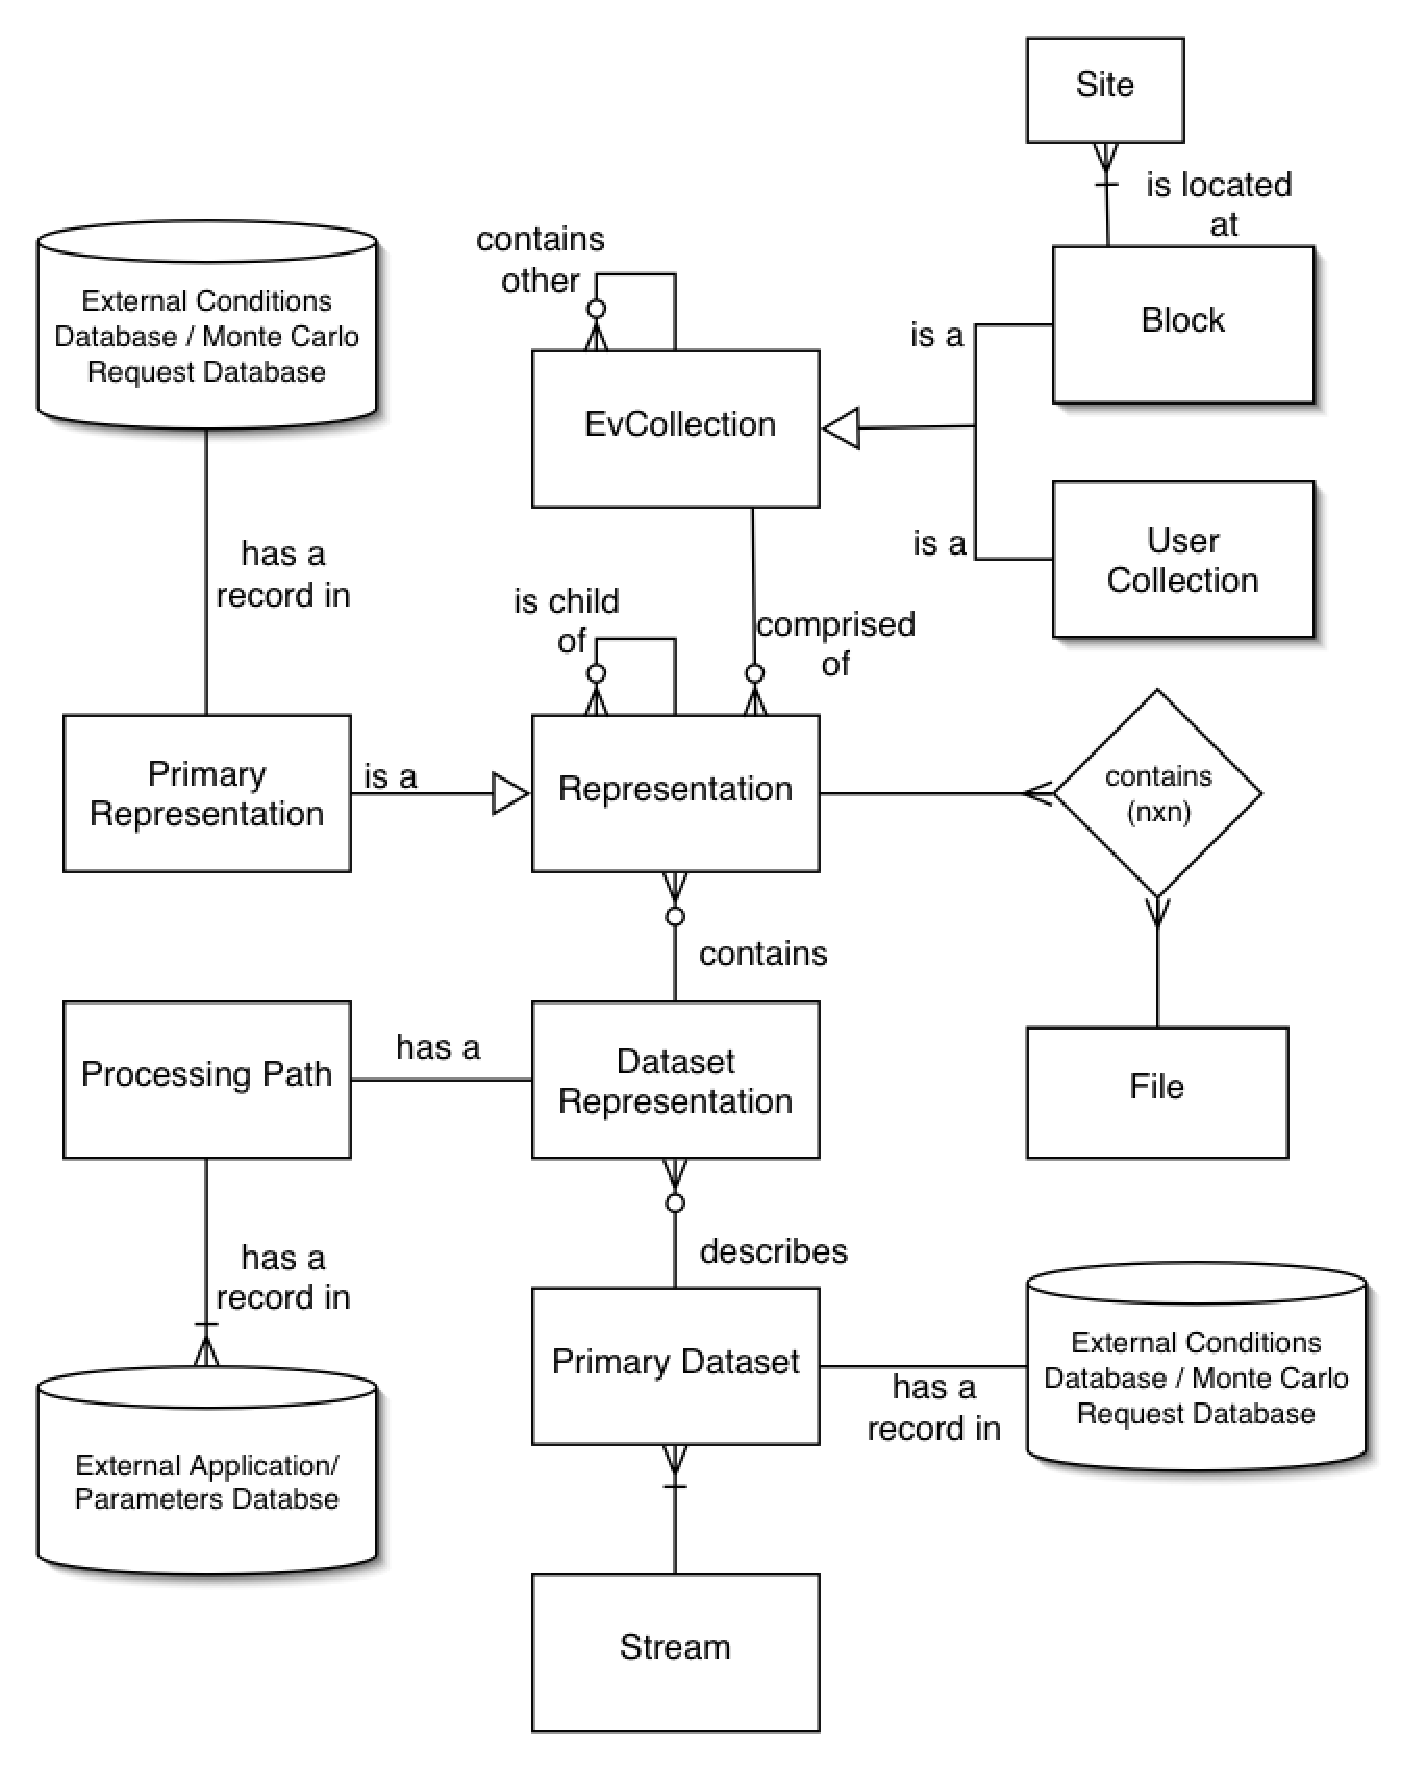
\includegraphics{DatasetBookkeeping-2a.eps}}
    \caption{A (nearly) complete schema.}
    \label{fig:detailed}
  \end{center}
\end{figure}
Two types of Event Collection are recognized here: blocks and user collections.  The 
notion of block has been put forward in order to better manage physical placement of data.  
Blocks are therefore distinguished by having a one to many relationship to a supporting site 
entity.  It is furthermore proposed that blocks satisfy the constraint that they be 
partitions on the Dataset Representation in the sense that no event IDs
can exist in two different blocks of the same type (as determined by the paths of the 
corresponding Event Collections.) This greatly simplifies the task of deciding which 
blocks to transfer given a set of interesting Event Collections.
Blocks are special in that they represent a new implementation detail 
that must be hidden from the physicist.  However, block constraints and behavior can be 
hidden in an application layer.  Finally, the recursion in Event Collection 
addresses oddities may arise 
because the scale introduced by blocksize and number of blocks per dataset may change.  
If one introduces blocks in order to deal with data on a given scale, one someday may need 
to introduce "super-blocks" if that scale changes, and so on. 

User collections are a type of Event Collection that supports the idea that users can specify 
collections of interest.  User collections are just a list of Event Collections
and can span multiple blocks.  
In order to be able to include references to pre-existing user collections, recursion is 
envisaged.  We can use the user collection to support a snapshot of the data, for example 
a collection of blocks in a streamed dataset that does not change or grow as the dataset 
grows.  Also, the data associated with a RefDB production assignment can also be supported 
as a special kind of user collection.


\subsection{Even more detail -- tables and attributes}

An initial set of attributes has been explored.  The file entity should contain obvious 
file attributes, such as logical filename, file size, cardinal times like creation and 
last access times, and checksum.  It should not contain site information, nor should 
site information at the file level be kept in this database schema.  Rather, it is 
thought that this information can be provided by external tools, and checked in an 
external validation tool is desired.  Only logical filenames will be tracked. One 
class of attributes we have not explored is access control.  It should be revisited later.

The Representation entity should contain brief and essential attributes such as run number, 
number of events in the collection, cardinal times like creation and access times, 
and a run status flag.  However, run conditions and calibration should probably 
be kept in  an external conditions or calibration database.  Pointers can be kept 
into those databases and vice-versa.  Part of the primary key of the Representation
should be the Primary Dataset that the Representation 
belongs to as well as the complete processing path.  This should be a unique key of 
Dataset Representation.  

Blocks should contain a unique block id that identifies its partition, and should 
have a block size and other low level metadata related to implementation.  Blocks 
should not contain physics metadata.  One of the special attributes needed in a 
block is a flag to indicate whether or not it is open for writing.  This will be 
explored in the next section.  Basically, in order to simplify the bookkeeping 
associated with having blocks, it will be a requirement that open blocks be 
restricted to a single site.  This has obvious implications for streaming, and 
can be dropped or revisited. 

The Dataset Representation table should contain Primary Dataset and processing path 
attributes to identify the Dataset Representation.  
Like blocks, it should also contain a flag indicating whether or not the Dataset Representation 
is open for writing.  A potential complication is the attribute 
difference between Monte-Carlo and real data 
datasets.  It is felt however that the differences in attributes can be expressed in support 
tables.  The attributes need to indicate Monte-Carlo or real.  In 
addition, quantities that need to be searchable should be included directly here.  However, 
blob data (non-queryable binary large objects such as compressed logs) can also be kept for provenance 
purposes.  

Event Collections can contain further attributes.  User collections should for 
example contain annotations indicating why they were created.  Blocks contain 
pointers to sites.  Collections corresponding to assignment IDs could contain pointers 
into the RefDB plus some metadata for querying.

Storage of attributes supporting the various 
entities in the proposed schema can be implemented as support tables.  The support table 
is a basic ER design pattern which allows metadata to be stored in a queryable format 
outside of the table directly representing the entity.  Attributes such as generation and 
simulation parameters for Monte-Carlo to run status information can be kept in support 
tables.   The support tables for the proposed schema have not been drawn for simplicity.  
Each principal entity in the schema should probably have a support table.

\subsection{Creating an Event Collection from another Event Collection}
\label{sec:createEvColl}

The input to a user Application is the Event Collection, and Event Collections can be 
created as the result of processing other Event Collections.  We examine a few cases 
here to illustrate how these processing results can be recorded using the DBS schema.
Below, we make casual use of the ``Run'' construct again.  However, ``Run'' can be replaced
by whatever data unit is actually used.  In the following,
it can be safely assumed that the relation between Event Collection and Representation 
(figure \ref{fig:highlevel}) can have an attribute that tells the application how to select 
out the data associated with the Representation given the whole Event Collection as
input.  

\subsubsection{Processing a Single Unit of Data}

A trivial case is where the Event Collection consists of a single Representation. 
This could be, for example, a single run.  The job processes the Event Collection 
and produces an output Event Collection.  The output Event Collection is associated 
with newly produced files.  The new files are stored back into the DBS as a child 
Representation of the input,  and the output Event Collection has this Representation 
as its sole member. 

\subsubsection{Processing Multiple Units of Data}

In this case, the event collection consists of multiple Representations. This 
could be for example multiple runs.  If each component Representation can be 
processed by a single job\footnote{The actual condition here is that the processing 
of an input Representation produces a distinct set of files, up to a few common ``metadata'' 
files.}, then as in the above case of a single Run, the results
can be stored back into the system as child representations and then grouped
together to form an output Event Collection.  

\subsubsection{Filtering: Multiple Units of Data Input and Single Unit Output}

In this case, we assume that the output Event Collection, though produced with
many inputs, is become whole in that it is not useful (nor in some cases 
even possible) to subdivide the output Event Collection in terms of the 
index used to define the input Representations.  For example, if the input is 
a list of runs and the  output is a single colletcion consisting of a few 
events from each run selected according  to some physics criterion. We 
assume that the output is a set of files for which there is no map
showing which files contain which events.  Then there are two choices.
\begin{enumerate}
\item Store the output back into the system as a single Representation with 
the output Event Collection containing only that Representation.  Either it 
is stored as a new Primary Representation and some limited parentage information 
is kept in the form of a parent Event Collection attribute,  or it 
could also be allowed that a child can have many parents and then the strict 
tree structure is destroyed.  (Kudzu vine structure?) 
\item For each input Representation, create a child Representation that points 
to the same entire set of files comprising the output Event Collection.  This
would preserve the tree structure and all of the relationships and might 
result in faster queries.  
\end{enumerate}
More thought is needed as to the best way to do this.  More than one way could be 
supported.  

\subsubsection{Mixing: Multiple Units of Data Input and Multiple Mixed Outputs}

In this case, we assume mixing is going on.  For exampe, the input could be 
an Event Collection comprising Representations according to $N$ runs and the 
output could be an Event Collection according to $M$ luminosity bins.  This 
can be achieved as a duplication of the above case on filtering by 
considering each output bin as corresponding to its own filter.  
\begin{enumerate}
\item Store the reclustered events back into the system as multiple 
Representations, each one corresponding to a luminosity bin in the example. 
The output EventCollection is the collection of all such Representations.
As above, these could be new Primary Representations or multi-parented.
\item For each output Representation, and then for each input Representation
contributing to that output Representation, create a child Representation 
that points to the same entire set of files comprising the output Representation.
The entire collection then becomes the output Event Collection.  
\end{enumerate}
More thought is needed as to the best way to do this.  More than one way could be 
supported.  For example, the first option is probably more efficient in terms of 
space, but less efficient in terms of queries on the parentage information.

\section{Architecture}


At the top of the application stack is the application database server layer which contains
the application logic.  (NB- This layer abstracts the clients from the schema and is not 
to be confused with the database server proper such as Oracle which serves SQL requests.) 
The database server layer manages the API that user applications will see.  It needs to 
support basic use cases of queries against the underlying database, such as discovering 
datasets from metadata or asking for the number of events in a given run range.  It 
should also support an API to get the information needed to initiate an analysis.  

The dataset bookkeeping service (DBS) proper is kept immediately below the database 
server layer.  The dataset bookkeeping service was split into the "canonical" dataset 
bookkeeping service (DBS) plus a dataset replica service(DRS).  This reflects the 
desire to keep replica locating functionality out of the DBS altogether is possible, 
and in a separate schema if absolutely necessary.    We agreed that if fine grained 
site information was included, then access to site information (DRS) should be kept 
decoupled as possible from the actual core dataset bookkeeping functionality (DBS), 
hence the two interfaces in the diagram.  (This is a somewhat arbitrary distinction, 
and maybe it goes away upon further inspection.)

\begin{figure}[hbtp]
  \begin{center}
    \resizebox{6cm}{!}{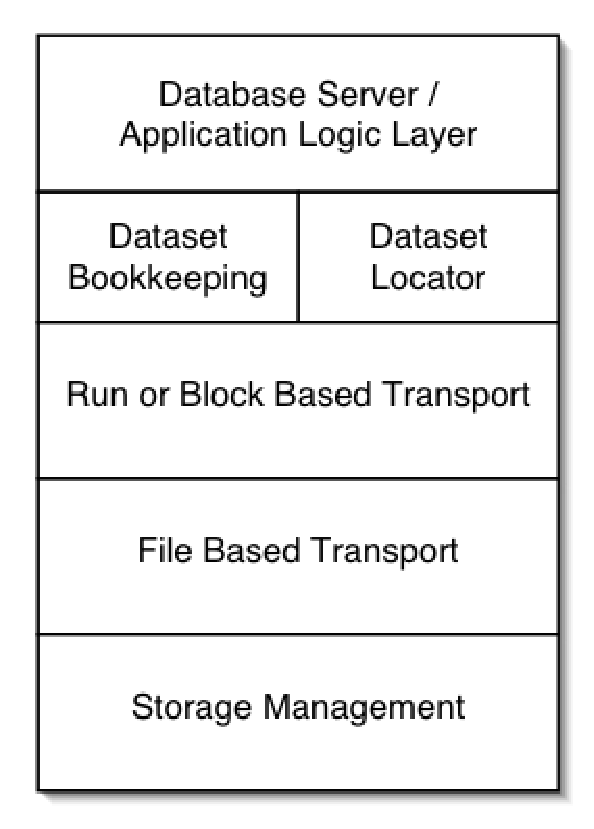
\includegraphics{DatasetBookkeeping-3a.eps}}
    \caption{}
    \label{fig:ex3}
  \end{center}
\end{figure}

Next, there is a layer specializing in Run and/or Block data transport.  
This layer can contain primitives and checks that guarantee transport of 
runs and/or blocks.  Underneath are file and storage infrastructure layers.

\subsection{Distributed Databases}

We did not explore the ramifications of distributing the database on the above schema.  
We briefly explored what it would mean to transfer a block to a site that was maintaining 
its own copy of the DBS.  We suspect that the corresponding runs would not have to be 
re-imported at that time.  Rather, we imagine that the corresponding data would be added 
to the local database through a lower level interface layer.  Important questions remain:  
is the block ID unique throughout all instances of a DBS?  What is the exact workflow for 
replicating a block?   After some discussion, we were nonetheless confident that the 
proposed schema with the addition of some transfer protocols would be sufficient.  
(To be expanded.) 

\section{Other Considerations}

Runs have a fill structure.  We do not at this time believe that substructure within 
runs need be tracked by this schema.  We prefer to imagine that a run conditions 
database will keep track of how run conditions change in a regular way taking into 
account a known fill structure.  Runs will change when irregularities occur and cause 
the operators to shut down the current run and start a new one.  

At this time, we do not foresee the need to create a dataset from a 
pre-existing Event Collection.  In our current model, a dataset must be created 
before one can add data to it, and therefore all of the Event Collections must 
already comprise data that belongs to a dataset.  


\appendix

\section{Addendum on Data ``Sets''}

In order to clarify the relationships between the given entities given in the main part of 
this note, it was felt that some formulae would help. 

\subsection{Representations and Datasets}

\begin{enumerate}

\item {\bf A Primary (or Production) Dataset $\Delta$} 
contains all data that shares certain physics 
attributes such as trigger bits or generation channels.  For example, ``Higgs to 2 electron''
or ``W to e nu'' or some other physics channel or trigger or luminosity condition.  (We omit 
here an index spanning the roughly 50 various trigger bits/channels to be present in the 
real data.) 

\item {\bf A Processing Path $\pi$} is a sequence of applications with version imformation 
and invocation parameters that
characterizes the provenance of processed data.  The null path $\emptyset$ contains
no applications and represents ``raw data'' in the sense that it is unprocessed.  

\item {\bf A Dataset Representation $\Delta_{\pi}$} is a selection of data within a primary 
dataset $\Delta$ that contains only data that has the provenance $\pi$.  For example, 
``Digi data'' within $\Delta$ is $\Delta_{\mbox{Digi}}$.  Of course, the provenance specification 
can be as complicated as you wish.

\item Let $\Pi(\Delta)$ be the collection of all processing paths defined for a Primary 
Dataset $\Delta $.  Then 
\begin{equation}
    \Delta = \{ \Delta_{\pi} \mid \pi \in \Pi(\Delta) \}
\end{equation}

\item $\Delta_{\emptyset}$ refers to the raw data in $\Delta$. (Or unprocessed data for 
Monte Carlo data.) 

\item Let $\rho$ index units of data $\Delta_{\emptyset}^{\rho}$ 
in $\Delta_{\emptyset}$.  The unit 
could be a Monte Carlo run, it could be a raw data run, 
it could be a luminosity bin within a raw data run, 
individual events, etc.  Let $R(\Delta)$ be the 
set of all such indices in $\Delta$.

\item A {\bf Data Unit Representation} $\Delta_{\pi}^{\rho}$ is the 
data in $\Delta$ that corresponds to the result of processing $\Delta_{\emptyset}^{\rho}$ 
through the given path $\pi$.  

\item The union
of all Representations of data units at a at some path $\Delta_{\pi}^{\rho}$ is 
\begin{equation}
\bigcup_{\rho \in R(\Delta)} \Delta_{\pi}^{\rho} = \Delta_{\pi}
\end{equation}
which is just another way of writing the Dataset Representation.  

\item A Representation $\Delta_{\pi}^{\rho}$ can 
be considered to be a node of data in a processing tree.  
The root node of such a tree is the {\bf Primary Representation} $\Delta_{\emptyset}^{\rho}$ 
of the unit of data.  The Primary Representation can correspond to a 
run of raw data, for example, or some other unit of data 
(other than a run) to be determined.  

\item The whole processing tree in $\Delta$ rooted 
at $\rho$ can be represented as $\Delta^{\rho}$. 
\begin{equation}
\Delta^{\rho} = \{ \Delta_{\pi}^{\rho} \mid \pi \in \Pi(\Delta) \}
\end{equation}

\item To get the Primary Dataset back again, 
\begin{equation}
\Delta = \bigcup_{\rho \in R(\Delta)} \Delta^{\rho} = \bigcup_{\rho \in R(\Delta)} \{ \Delta_{\pi}^{\rho} \mid \pi \in \Pi(\Delta) \} 
\end{equation}

\end{enumerate}


\subsection{Event Collections}

And for Event Collections, which are meant to be more flexible and user definable: 

\begin{enumerate}

\item Defining an Event Collection as a collection of Representations of units of data.  
Consider some
subset $R_I$ of data indices of interest in $R(\Delta)$:  $R_I \subseteq R(\Delta)$.
Say one is interested only in 
data processed through some concrete path $\pi$.  An Event Collection $\xi_{\pi}^{R_I}$
can be defined as 
\begin{equation}
\xi_{\pi}^{R_I} = \bigcup_{\rho \in R_I} \Delta_{\pi}^{\rho}
\end{equation}

\item Of course, one special case is a Dataset Representation. 
\begin{equation} 
\xi_{\pi}^{R(\Delta)} = \Delta_{\pi}
\end{equation}


\item Definition of a partition into $N$ disjoint $P_N$ on a set $X$ : 
$ P_N = \{ y_i \mid i = 1...N, y_i \subset X \} $ such that 
\begin{equation}
\bigcup_{i=1}^N y_i = X
\end{equation} 
and 
\begin{equation} 
y_i \cap y_j \neq \emptyset \mbox{ if and only if } i = j
\end{equation}
 
\item  Another special case of Event Collection 
is for ``blocks'', or ``dataset partitions''.  For example, if
$P_N = \{ p_i \}$ is a partition over $R(\Delta)$ of size $N$, then : 
\begin{equation}
B_{\pi} = \{ \xi_{\pi}^{p_i} \mid i = 1...N\}
\end{equation}
is a set of ``blocks'' of data of type $\pi$.  For raw data, $\pi = \emptyset$.


\item Let $\Pi_J$ define some collection of interesting processing paths, like ``Hits and Digis'', 
in $\Pi(\Delta)$.  Let a Compound Representation $C_{\Pi_J}^{\rho}$ be defined by
\begin{equation}
C_{\Pi_J}^{\rho} = \{ \Delta_{\pi}^{\rho} \mid \pi \in \Pi_J \}
\end{equation}
In the E-R schema provided in the document, the Compound Representation should be 
represented in the self-relation on the Representation entity.  We draw attention to 
this distinction here for clarity.

\item Defining an Event Collection as a collection of compound Representations: 
\begin{equation}
\xi_{\Pi_J}^{R_I} = \bigcup_{\rho \in R_I} C_{\Pi_J}^{\rho} = \bigcup_{\rho \in R_I} \{ \Delta_{\pi}^{\rho} \mid \pi \in \Pi_J \}
\end{equation}

\item Blocks can be defined similarly over Compound Representations if the $R_I$ are a partition 
of $R(\Delta)$.

\end{enumerate}

All types of entities above can be represented in the provided schema.  (Or the schema
is in error.)  The Event Collection can be understood as a cartesian product of some
``results of processing'' and some ``units of interesting data''.  

\subsection{Error in Terminology}

Previous versions ($\le 0.3$) of this document contained the following accidental obfuscation.  
Partitioning a dataset ``horizontally'' means that the partitions should have something 
to do with an event aggregate index, like a run number.  Horizontal partitions should 
thus contain events.  Aggregating data horizontally means that the 
event aggregate index (or run number) is ``summed out'' of the reference.  Aggregation 
is thus complementary to partition.  

In the referenced documents, the sense that the EventCollection entity 
partitions the data ``horizontally'' was reversed in this way.  EventCollection really 
aggregates the data ``horizontally'', and Representation aggregates the data ``vertically''
(or according to data type.)  

We apologize for any confusion.


\begin{thebibliography}{9}
  \bibitem{dmman} The DM.txt document, being migrated into the Computing
      TDR (CTDR) document repository
  \bibitem{rtag7} {\bf CMS Internal Note 2004/038}, R. Harris et al., 
    {\it Report of the CMS Data Management RTAG}

  \bibitem{CM} {\bf CMS Note 2004/031}, C. Grandi, D. Strickland,
               L. Taylor, {\bf The CMS Computing Model}

  \bibitem {NOTE000} {\bf CMS Note 2005/000},
    X.Somebody et al.,
    {\em "CMS Note Template"}.
\end{thebibliography}
 
%------------------------------------------------------------------------------
\pagebreak

\end{document}
